\documentclass{article}
\usepackage[utf8]{inputenc}
\usepackage{amsmath,amsfonts,amssymb,amsthm,mathtools}
\usepackage{parskip}
\usepackage{color}
\usepackage{booktabs}
\usepackage{hyperref}
\usepackage{tikz}
\usepackage[framemethod=tikz]{mdframed}
\usepackage{float}
\usepackage{placeins}
\usepackage{subcaption}
\usepackage{graphicx}

\definecolor{blue}{RGB}{38,139,210}
\definecolor{cyan}{RGB}{42,161,152}
\definecolor{violet}{RGB}{108,113,196}
\definecolor{red}{RGB}{220,50,47}
\definecolor{base01}{RGB}{88,110,117}
\definecolor{base02}{RGB}{7,54,66}
\definecolor{base03}{RGB}{0,43,54}

\usetikzlibrary{calc,shapes,positioning}

\newtheorem{exercise}{Exercise}
\newtheorem{answer}{Answer}

\newcommand{\dd}[2][]{\frac{\partial #1}{\partial #2}}
\newcommand{\dt}[2][]{\frac{d #1}{d #2}}
\newcommand{\dL}{\dt[{\L}]}
\newcommand{\dLi}{\dt[{\Li}]}
\newcommand{\dLmb}{\dt[{\Lmb}]}
\newcommand{\dLfb}{\dt[{\Lfb}]}
\newcommand{\yh}{\hat{y}}

\newcommand{\bracket}[3]{\left#1 #3 \right#2}
\newcommand{\sqb}{\bracket{[}{]}}
\newcommand{\ab}{\bracket{\langle}{\rangle}}
\renewcommand{\b}{\bracket{(}{)}}
\newcommand{\abs}{\bracket{\lvert}{\rvert}}

\newcommand{\W}{\mathbf{W}}
\renewcommand{\a}{\mathbf{a}}
\newcommand{\h}{\mathbf{h}}
\newcommand{\p}{\mathbf{p}}

\newcommand{\Cin}{C_\text{in}}
\newcommand{\Cout}{C_\text{out}}
\newcommand{\Win}{W_\text{in}}
\newcommand{\Wout}{W_\text{out}}
\newcommand{\Wk}{W_\text{kernel}}
\newcommand{\Hin}{H_\text{in}}
\newcommand{\Hout}{H_\text{out}}
\newcommand{\Hk}{H_\text{kernel}}



\title{EMAT31530: Convolutional neural networks}
\author{Laurence Aitchison}
\date{}

\begin{document}

\maketitle

So far, we've seen lots of material on how to train NNs using backprop, and how to use PyTorch.
But to actually apply NNs to e.g.\ image datasets (for instance for classifying the objects in the image), we need to consider architectures specifically adapted to images.
Perhaps the key operation is ``convolution'', which is the basis for all the classic and many of the modern networks for images.
Networks that involve convolutional layers are called ``convolutional neural networks'', and that's what we'll look at this week!


\section{Images and feature maps as tensors}

To understand convolutions, the first step is to understand how we represent images in deep learning.
We represent images as big 3D tensors, with shape $3 \times \text{height} \times \text{width}$,

\begin{center}
  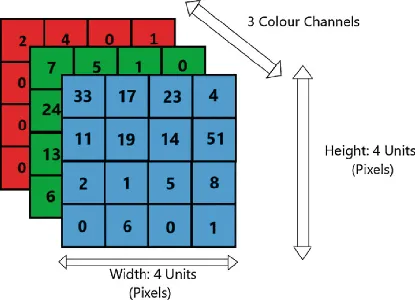
\includegraphics[width=0.5\textwidth]{image_as_tensor.png}
\end{center}

The three colour channels represent the red, green and blue channels in the image (i.e. the amount of red, green or blue at that pixel).
Alternatively, a greyscale image is a $1 \times \text{height} \times \text{width}$ image.

A feature map is very similar to an image. 
The key difference is that a feature map has much larger number of channels (usually around 100 -- 500), rather than 3 in a colour image or 1 in a greyscale image.
So a feature map is of shape $\text{channels} \times \text{height} \times \text{width}$, which is usually abbreviated to $C\times H \times W$.
You can imagine that in a feature map, we have assigned a feature vector to every pixel in every image.
That contrasts to fully-connected networks, where we'd just have one feature vector associated with every image.

In practice, we usually work with a minibatch of $N$ images. 
Thus, we end up working with tensors of size $\text{minibatch size} \times \text{channels} \times \text{height} \times \text{width}$, which is usually abbreviated to $N \times C\times H \times W$.

Convolutional layers take images/feature maps as inputs, and returns images/feature maps as outputs.
We'll see how they operate in the next section.


\clearpage
\FloatBarrier
\section{Convolutions}

To start, we draw a diagram for the simplest possible deep-learning style convolution.
Specifically, consider a convolution with one input channel and one ouput channel, and with convolutional weights (or ``kernel''),
\begin{figure}[H]
    \centering
    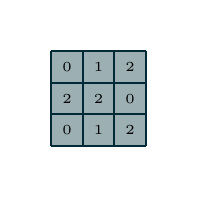
\begin{tikzpicture}[scale=.4,every node/.style={minimum size=1cm}, on grid]
            \draw[fill=base02,opacity=0.4] (0,0) rectangle (3,3);
            \draw[draw=base03,thick] (0,0) grid (3,3);
            \node (00) at (0.5,2.5) {\tiny 0};
            \node (01) at (1.5,2.5) {\tiny 1};
            \node (02) at (2.5,2.5) {\tiny 2};
            \node (10) at (0.5,1.5) {\tiny 2};
            \node (11) at (1.5,1.5) {\tiny 2};
            \node (12) at (2.5,1.5) {\tiny 0};
            \node (20) at (0.5,0.5) {\tiny 0};
            \node (21) at (1.5,0.5) {\tiny 1};
            \node (22) at (2.5,0.5) {\tiny 2};
    \end{tikzpicture}
\end{figure}
These weights are $3 \times 3$, so we say that the ``kernel size'' is 3.

We slide these weights over the input image/feature map.
At each location, we calculate the product between the weight and the image pixel.
We sum all these products to get the output in the current location.
\begin{figure}[H]
    \centering
    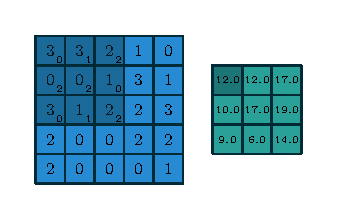
\includegraphics[width=0.32\textwidth]{pdf/numerical_no_padding_no_strides_00.pdf}
    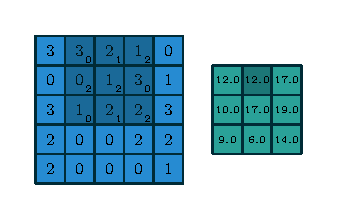
\includegraphics[width=0.32\textwidth]{pdf/numerical_no_padding_no_strides_01.pdf}
    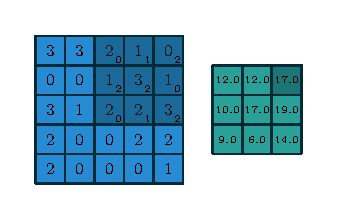
\includegraphics[width=0.32\textwidth]{pdf/numerical_no_padding_no_strides_02.pdf}
    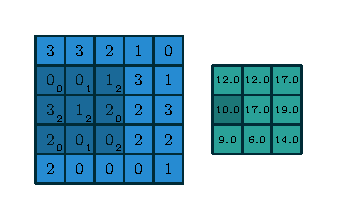
\includegraphics[width=0.32\textwidth]{pdf/numerical_no_padding_no_strides_03.pdf}
    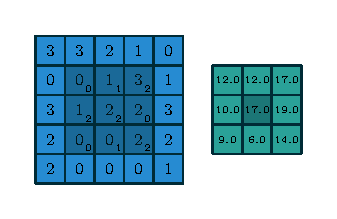
\includegraphics[width=0.32\textwidth]{pdf/numerical_no_padding_no_strides_04.pdf}
    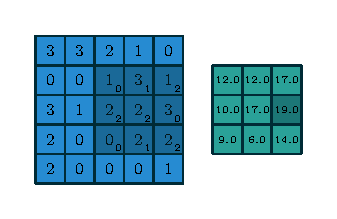
\includegraphics[width=0.32\textwidth]{pdf/numerical_no_padding_no_strides_05.pdf}
    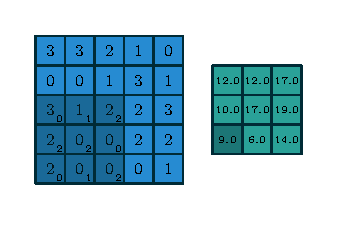
\includegraphics[width=0.32\textwidth]{pdf/numerical_no_padding_no_strides_06.pdf}
    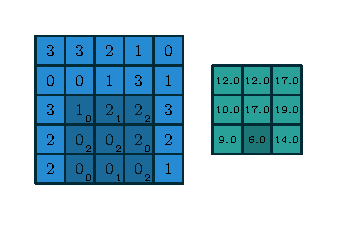
\includegraphics[width=0.32\textwidth]{pdf/numerical_no_padding_no_strides_07.pdf}
    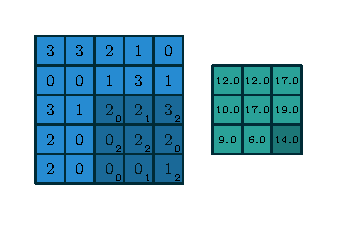
\includegraphics[width=0.32\textwidth]{pdf/numerical_no_padding_no_strides_08.pdf}
    \caption{\label{fig:numerical_no_padding_no_strides} 
      Computing the output of a simple convolutional layer.  The blue $5 \times 5$ square shows the inputs, the green $3 \times 3$ square shows the output.  The darker $3\times 3$ square in the input shows the current location of the patch of weights as it slides over the image.  This diagram along with others in this pdf are taken from ``A guide to convolution arithmetic for deep learning'', by Vincent Dumoulin and Francesco Visin.  This is a great article to check out if you're interested in filling in any gaps.
    }
\end{figure}
Specifically, the formula for this simple convolution is,
\begin{align}
  \label{eq:conv2d_scalar}
  a_{x,y} &= \sum_{\delta_x=-1}^1 \sum_{\delta_y=-1}^1 h_{x+\delta_x, y+\delta_y} W_{\delta_x, \delta_y}
\end{align}
here:
\begin{itemize}
  \item $a_{x, y}$ is the output image / feature map. In this example, the outputs are size $3\times 3$. So the indices $x$ and $y$ represent location in the output image, and range from $1$ to $3$.  As an example, looking at the previous diagram, and starting our indexing in the top-left, $a_{1, 1} = 12.0$.
  \item $h_{x+\delta_x, y+\delta_y}$ is the input image / feature map. In this example, the inputs are size $5\times 5$.  So the indices $x + \delta_x$ and $y + \delta_y$ represent location on the input image, and range from $0$ to $4$.  As an example, looking at the previous diagram, and starting our indexing in the top-left, $h_{0, 0} = 3$.
  \item $W_{\delta_x, \delta_y}$ is the convolutional weights (in grey in the first image, or in the $3 \times 3$ darker patches in the inputs in Fig.~\ref{fig:numerical_no_padding_no_strides}).  In this example, the weights are size $3 \times 3$. So the indicies $\delta_x$ and $\delta_y$ represent the location within the $3 \times 3$ weight matrix, and range from $-1$ to $1$. As an example, looking at the previous diagram, and starting our indexing in the top-left, $W_{-1, -1} = 0$.
\end{itemize}
Note that here, when we say that ``an index ranges from $-1$ to $1$'', we're being flexible for the purposes of making the maths easy.
In Python/PyTorch, indicies always range from $0$ to $(\text{length}-1)$.

There are a coupple of ways of interpreting a convolution in terms of matrices and vectors.
Both of these interpretations are easier to understand if we consider a 1D convolution, where instead of the inputs and outputs being images with 2 spatial dimensions, they just have one spatial dimension, $x$.
In that case, Eq.~\eqref{eq:conv2d_scalar} becomes,
\begin{align}
  \label{eq:conv1d_scalar}
  a_{x} &= \sum_{\delta=-1}^1 h_{x+\delta} W_{\delta}.
\end{align}
Writing out the individual components (for a length five input and a length three output),
\begin{align}
  \label{eq:conv1d_scalar_sum}
  a_{x} &= W_{-1} h_{x-1} + W_0 h_x + W_1 h_{x+1}
\end{align}
or,
\begin{subequations}
\label{eq:conv1d_scalar_components}
\begin{align}
  a_1 &= h_0 W_{-1} + h_1 W_{0} + h_2 W_{1}\\
  a_2 &= h_1 W_{-1} + h_2 W_{0} + h_3 W_{1} \\
  a_3 &= h_2 W_{-1} + h_3 W_{0} + h_4 W_{1}
\end{align}
\end{subequations}

\subsection{Interpretation 1: linear operation on patches}
Notice that the components in Eq.~\eqref{eq:conv1d_scalar_sum} can be written as a big matrix operation,
\begin{align}
  a_{x} &= 
  \underbrace{\begin{pmatrix}
    h_{x-1} &
    h_{x} &
    h_{x+1}
  \end{pmatrix}
  }_{=\p_x}
  \underbrace{\begin{pmatrix}
    W_{-1} \\
    W_{0} \\
    W_{+1}
  \end{pmatrix}}_{=\W}
  = \p_x \W
\end{align}
Here, $\p_x$ is the inputs in the patch around $h_x$ concatenated together
\begin{align}
  \p_{x} &= \begin{pmatrix} 
    h_{x-1} &
    h_{x} &
    h_{x+1}
  \end{pmatrix},
\end{align}
and $\W$ is the weights for all parts of the patch concatenated together,
\begin{align}
  \W &= \begin{pmatrix}
    W_{-1} \\
    W_{0} \\
    W_{1}
  \end{pmatrix}.
\end{align}


%Here, $\p_x$ is the represents inputs in the patch around $\h_x$ concatenated together.  Remember that $\h_{x}$, is a row vector of size $\Cin$, so $\p_{x}$ is a bigger row-vector, of length ($3 \Cin$).
%\begin{align}
%  \p_{x} &= \begin{pmatrix} 
%    h_{x-1} &
%    h_{x} &
%    h_{x+1}
%  \end{pmatrix}
%\end{align}
%Moreover, $\W$ is a joint matrix for all locations in the patch,
%\begin{align}
%  \W &= \begin{pmatrix}
%    W_{-1} \\
%    W_{0} \\
%    W_{1}
%  \end{pmatrix}
%\end{align}
%Remember that $\W_\delta$ is of size $\Cin \times \Cout$.  So $\W$ is a matrix of size $(3 \Cin)\times \Cout$. 
%Thus, $\W$ is the right shape to take whole patches, $\p_{x,y}$ (which are vectors of length $3 \Cin $) as inputs.


\subsection{Interpretation 2: linear operations on the input image}
There's an alternative interpretation, which doesn't require us to extract patches, $\p_x$, from the input image.
Specifically, we can write out the result of Eq.~\eqref{eq:conv1d_scalar_components} as an alternative big matrix-vector operation, with a structured weight matrix,
\begin{align}
  \begin{pmatrix}
    a_1 & a_2 & a_3
  \end{pmatrix}
  &= 
  \begin{pmatrix}
    h_0 & h_1 & h_2 & h_3 & h_4
  \end{pmatrix}
  \begin{pmatrix}
    W_{-1} &   0    &   0    \\
    W_{ 0} & W_{-1} &   0    \\
    W_{ 1} & W_{ 0} & W_{-1} \\
      0    & W_{ 1} & W_{ 0} \\
      0    &   0    & W_{ 1}
  \end{pmatrix}
\end{align}
Note that the input and output vectors here are just the standard single-channel input and output vectors, $\h$ and $\a$, so we can write this expression as,
\begin{align}
  \a &= \h 
  \begin{pmatrix}
    W_{-1} &   0    &   0    \\
    W_{ 0} & W_{-1} &   0    \\
    W_{ 1} & W_{ 0} & W_{-1} \\
      0    & W_{ 1} & W_{ 0} \\
      0    &   0    & W_{ 1}
  \end{pmatrix}.
\end{align}
In fact, all convolutions can be understood as matrix multiplications with structured weights.
That interpretation is okay in this simple setting, with one input and output channel, and one spatial dimension, but becomes quite complex as soon as you consider multiple input/output channels, or more than one spatial dimension.

\FloatBarrier
\subsection{Convolutions with multiple input and output channels}

In the previous section, we considered the simplest setting for convolutions, with a single input channel, and a single output channel.
However, in practice in deep learning, we almost always have multiple input and multiple output channels.
What happens in that setting?
Well, it is almost exactly the same as in the single-input and single-output channel settings, except: 
\begin{itemize}
  \item Instead of an scalar at each location in the input and output (i.e.\ $h_{x+\delta x,y+\delta y}$ and $a_{x,y}$), there's a whole feature \textit{vector} at each location, $\h_{x+\delta_x, y+\delta_y}$ and $\a_{x,y}$.
  \item Instead of just a scalar weight at each location in the patch (i.e.\ $W_{\delta_x, \delta_y}$) that there's a whole weight matrix, $\W_{\delta_x, \delta_y}$.
\end{itemize}
Overall, that means a 2D convolution, with multiple input and output channels can be written,
\begin{align}
  \a_{x,y} &= \sum_{\delta_x=-1}^1 \sum_{\delta_y=-1}^1 \h_{x+\delta_x, y+\delta_y} \W_{\delta_x, \delta_y}.
\end{align}
Here,
\begin{itemize}
  \item $\a_{x, y}$ is a row-vector of length $\Cout$ (or \verb|out_channels| in PyTorch).  There is one vector at each spatial location in the output.
  \item $\h_{x+\delta_x, y+\delta_y}$ is a row-vector of length $\Cin$ (or \verb|in_channels| in PyTorch).  There is one vector at each spatial location in the input.
  \item $\W_{\delta_x, \delta_y}$ is a matrix of size $\Cin \times \Cout$.  There is one of these matrices at each location in the patch.
\end{itemize}

%Interpretations 1 + 2 can also be extended to the multi-dimensional case, by directly swapping the scalar inputs/outputs/weights for their vector/matrix counterparts, but we're only going to look at extending interpretation 1.
%
%\subsection{Interpretation 1 in the multidimensional setting}
%
%A convolution with 1 spatial dimension, but multiple input and output channels looks like,
%\begin{align}
%  \label{eq:conv1d_vector}
%  \a_{x} &= \sum_{\delta=-1}^1 \h_{x+\delta} \W_{\delta}.
%\end{align}
%Notice that Eq.~\eqref{eq:conv1d_vector} can be written as a big matrix operation,
%\begin{align}
%  \a_{x} &= 
%  \begin{pmatrix}
%    \h_{x-1} &
%    \h_{x} &
%    \h_{x+1}
%  \end{pmatrix}
%  \begin{pmatrix}
%    \W_{-1} \\
%    \W_{0} \\
%    \W_{+1}
%  \end{pmatrix}
%  = \p_x \W
%\end{align}
%Here, $\p_x$ is the represents inputs in the patch around $\h_x$ concatenated together.  Remember that $\h_{x}$, is a row vector of size $\Cin$, so $\p_{x}$ is a bigger row-vector, of length ($3 \Cin$).
%\begin{align}
%  \p_{x} &= \begin{pmatrix} 
%    \h_{x-1} &
%    \h_{x} &
%    \h_{x+1}
%  \end{pmatrix}
%\end{align}
%Moreover, $\W$ is a joint matrix for all locations in the patch,
%\begin{align}
%  \W &= \begin{pmatrix}
%    \W_{-1} \\
%    \W_{0} \\
%    \W_{1}
%  \end{pmatrix}
%\end{align}
%Remember that $\W_\delta$ is of size $\Cin \times \Cout$.  So $\W$ is a matrix of size $(3 \Cin)\times \Cout$. 
%Thus, $\W$ is the right shape to take whole patches, $\p_{x,y}$ (which are vectors of length $3 \Cin $) as inputs.

\subsection{Shapes in PyTorch in practice}

Finally, it is worth mentioning the shape of the inputs and weights in actual convolutions in PyTorch.
\begin{itemize}
  \item The inputs and outputs are standard feature maps, of size $N \times \Cin \times \Hin \times \Win$ and $N \times \Cout \times \Hout \times \Wout$. Note that the inputs and outputs can be of different sizes (e.g.\ in Fig.~\ref{fig:numerical_no_padding_no_strides} we had $5 = \Hin = \Win$ and $3 = \Hout = \Wout$). Finally, $N$ is the minibatch size.
  \item The weights are of size $\Cout \times \Cin \times \Hk \times \Wk$, where $\Hk$ and $\Wk$ are the size of the convolutional patch (or ``kernel''); (in Fig.~\ref{fig:numerical_no_padding_no_strides} we had $3 = \Hk = \Wk$).
\end{itemize}

\subsection{Convolutions in (Engineering) Maths [Non-Examinable]}

If you have not encountered convolutions before, you can ignore this section.
However, if you have encountered convolutions before in an (Engineering) maths context, you might be slightly confused, as convolutions are typically defined as,
\begin{align}
  \label{eq:math_conv}
  a(x) &= \int_{-\infty}^\infty d\delta' \; h(x - \delta') \; w(\delta') 
\end{align}
Note that here, $\delta$ is a variable, not the Kronecker/Dirac delta.
This is an operator that takes two functions ($h$ and $w$) as input, and returns a function, $a$ as output.
This doesn't look much like the AI-version of convolution.
We can make it look at bit more similar by setting, $\delta = -\delta'$
\begin{align}
  a(x) &= \int_{-\infty}^\infty d\delta \; h(x + \delta) \; w(-\delta).
\end{align}
If we write down a discrete version of this expression, we get something that looks alot like an AI-style convolution,
\begin{align}
  a_{x} &= \sum_{\delta=-\infty}^\infty h_{x+\delta} W_{-\delta}.
\end{align}
There are two key differences:
\begin{itemize}
  \item Here, $\delta$ ranges from $-\infty$ to $\infty$.  In contrast, in AI (Eq.~\ref{eq:conv1d_scalar}), $\delta$ has a small range, e.g. often from $-1$ to $1$.
  \item Here, there's a $-\delta$ in $W_{-\delta}$, while in AI (Eq.~\ref{eq:conv1d_scalar}) there's no minus sign so we just have $W_\delta$.  It turns out that this doesn't matter in AI, as all the elements of the weight are learned.
\end{itemize}



\FloatBarrier
\clearpage
\subsection{Convolutional Strides and Padding}
When practically using convolutions in deep learning, there are a few options to set.
In particular, the ``kernel size'', ``strides'' and ``padding''.
Previously, we have used the simplest (but perhaps not most standard) setting of stride=1 and padding=0.

Kernel size is the spatial size of the patch of weights that we slide over the image.

Strides give the size of the ``jumps'' as we slide the weights over the input image: see examples below.
As such, $\Hout \approx \Hin/\text{stride}$ and $\Wout \approx \Win/\text{stride}$.

Padding is a region around the input image that we fill with zeros: see dashed border around the inputs in the examples below.
Without padding, the outputs will tend to be smaller than the inputs, even with stride=1.
That happened above in Fig.~\ref{fig:numerical_no_padding_no_strides}.

\begin{figure}[H]
    \centering
    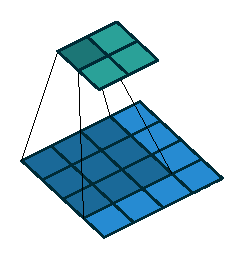
\includegraphics[width=0.24\textwidth]{pdf/no_padding_no_strides_00.pdf}
    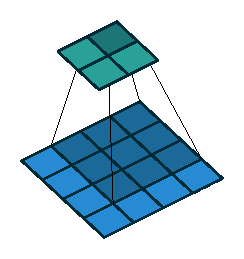
\includegraphics[width=0.24\textwidth]{pdf/no_padding_no_strides_01.pdf}
    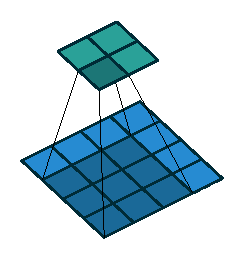
\includegraphics[width=0.24\textwidth]{pdf/no_padding_no_strides_02.pdf}
    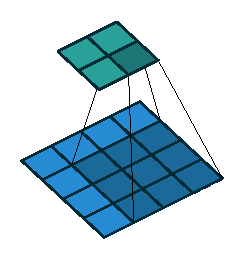
\includegraphics[width=0.24\textwidth]{pdf/no_padding_no_strides_03.pdf}
    \caption{\label{fig:no_padding_no_strides}
        Convolving a $4 \times 4$ input using kernel size=3, stride=1 and padding=0.}
\end{figure}

\begin{figure}[H]
    \centering
    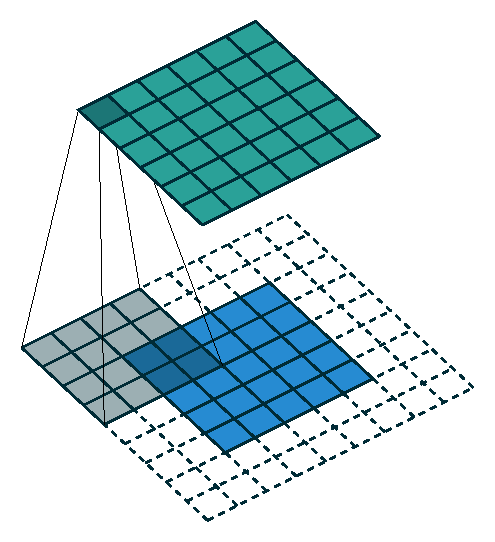
\includegraphics[width=0.24\textwidth]{pdf/arbitrary_padding_no_strides_00.pdf}
    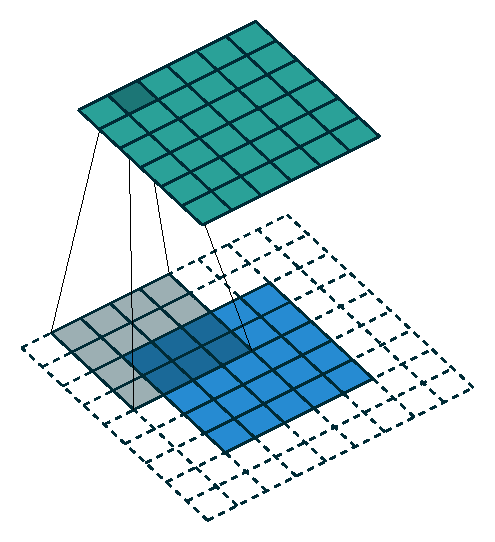
\includegraphics[width=0.24\textwidth]{pdf/arbitrary_padding_no_strides_01.pdf}
    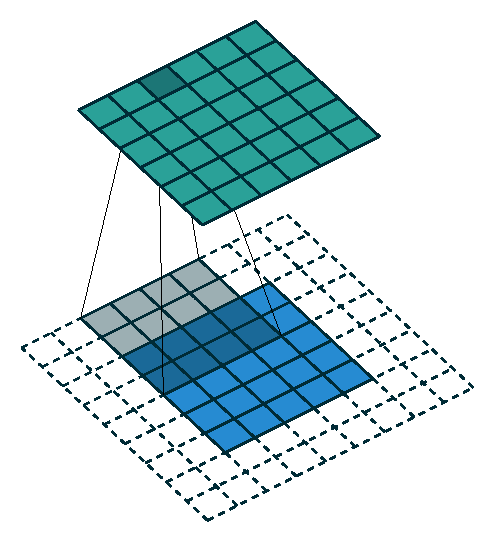
\includegraphics[width=0.24\textwidth]{pdf/arbitrary_padding_no_strides_02.pdf}
    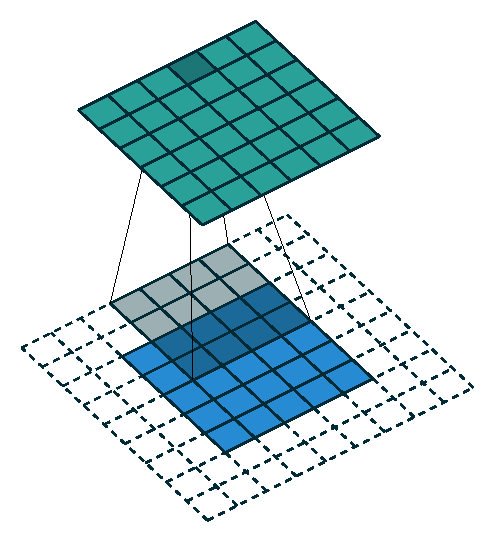
\includegraphics[width=0.24\textwidth]{pdf/arbitrary_padding_no_strides_03.pdf}
    \caption{\label{fig:arbitrary_padding_no_strides} 
        Convolving a $5 \times 5$ input using kernel size=4, stride=1 and padding=2.}
\end{figure}

\begin{figure}[H]
    \centering
    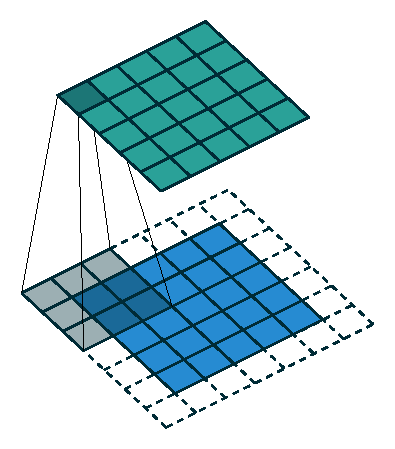
\includegraphics[width=0.24\textwidth]{pdf/same_padding_no_strides_00.pdf}
    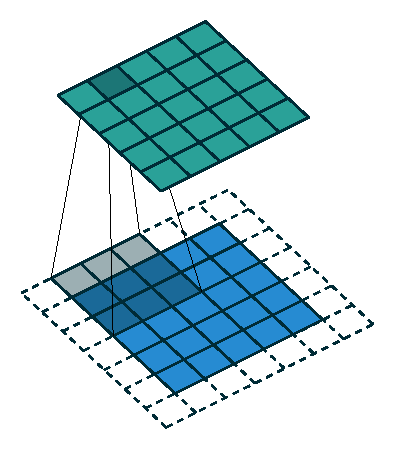
\includegraphics[width=0.24\textwidth]{pdf/same_padding_no_strides_01.pdf}
    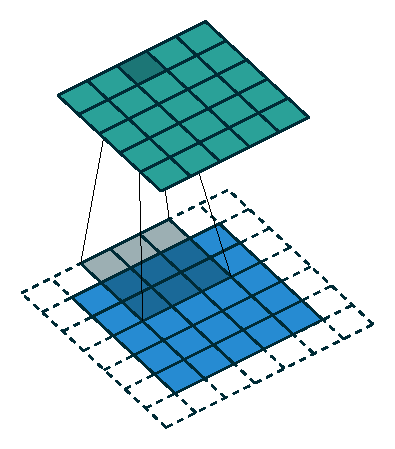
\includegraphics[width=0.24\textwidth]{pdf/same_padding_no_strides_02.pdf}
    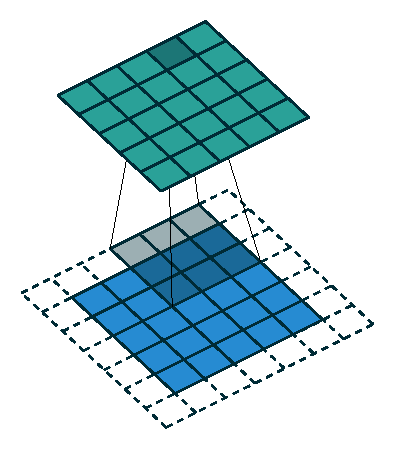
\includegraphics[width=0.24\textwidth]{pdf/same_padding_no_strides_03.pdf}
    \caption{\label{fig:same_padding_no_strides}
        Convolving a $5 \times 5$ input using kernel size=3, stride=1 and padding=1.
        Note this is known as ``same'' padding, as the input is the same shape as the output.}
\end{figure}

\begin{figure}[H]
    \centering
    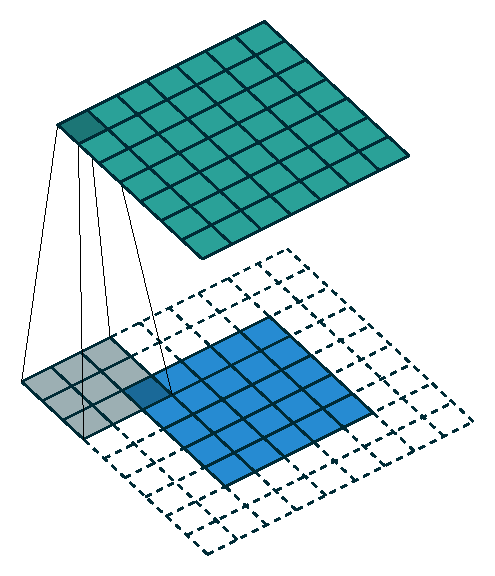
\includegraphics[width=0.24\textwidth]{pdf/full_padding_no_strides_00.pdf}
    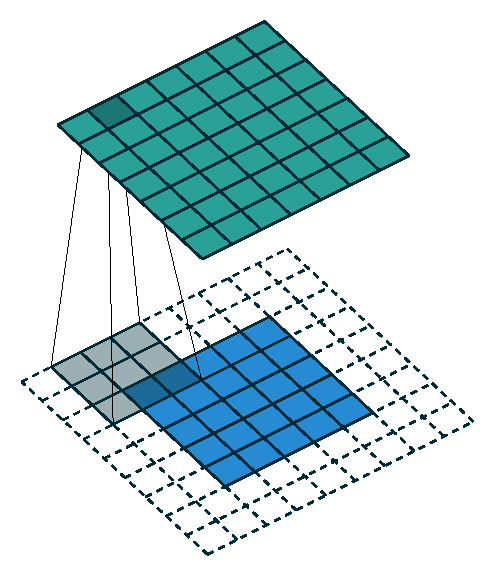
\includegraphics[width=0.24\textwidth]{pdf/full_padding_no_strides_01.pdf}
    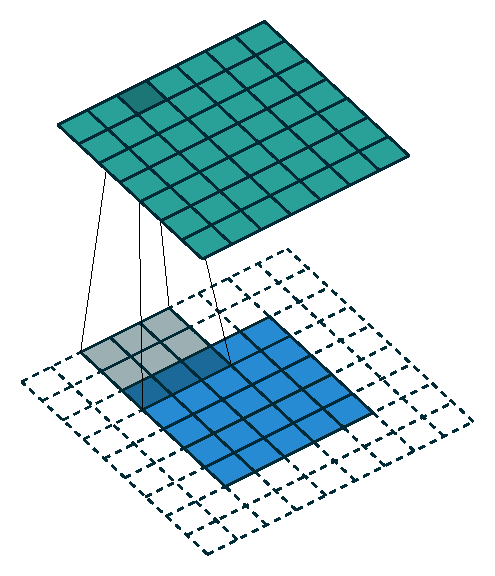
\includegraphics[width=0.24\textwidth]{pdf/full_padding_no_strides_02.pdf}
    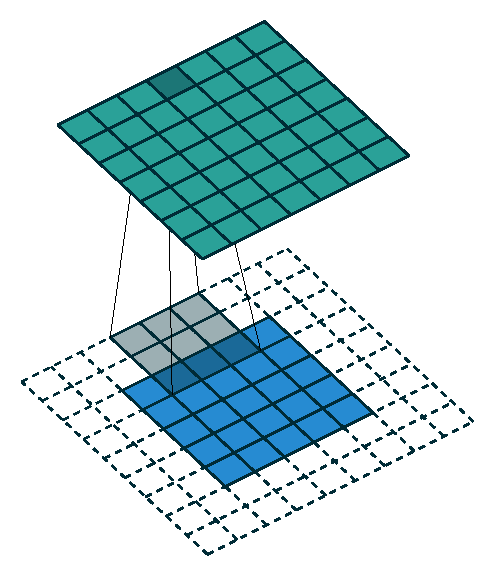
\includegraphics[width=0.24\textwidth]{pdf/full_padding_no_strides_03.pdf}
    \caption{\label{fig:full_padding_no_strides}
        Convolving a $5 \times 5$ input using kernel size=3, stride=1 and padding=2.}
\end{figure}

\begin{figure}[H]
    \centering
    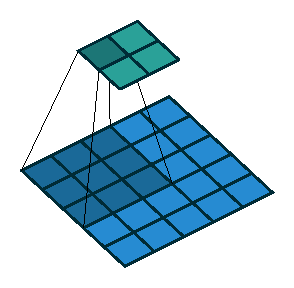
\includegraphics[width=0.24\textwidth]{pdf/no_padding_strides_00.pdf}
    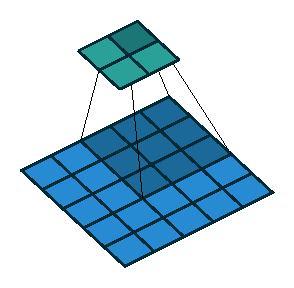
\includegraphics[width=0.24\textwidth]{pdf/no_padding_strides_01.pdf}
    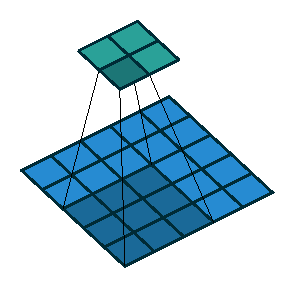
\includegraphics[width=0.24\textwidth]{pdf/no_padding_strides_02.pdf}
    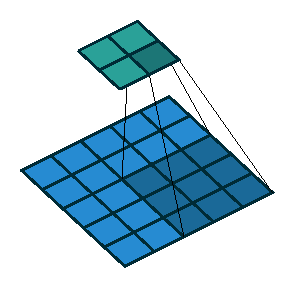
\includegraphics[width=0.24\textwidth]{pdf/no_padding_strides_03.pdf}
    \caption{\label{fig:no_padding_strides} 
        Convolving a $5 \times 5$ input using kernel size=3, stride=2 and padding=0.}
\end{figure}

\begin{figure}[H]
    \centering
    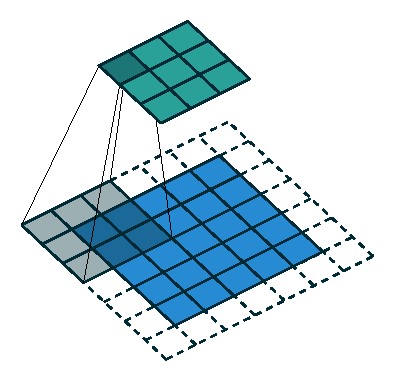
\includegraphics[width=0.24\textwidth]{pdf/padding_strides_00.pdf}
    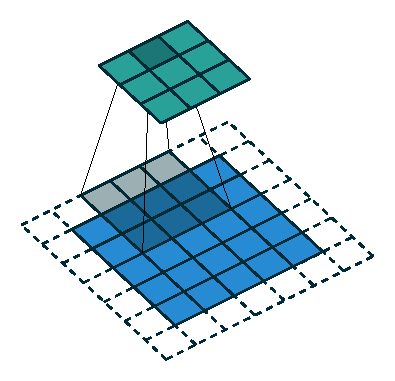
\includegraphics[width=0.24\textwidth]{pdf/padding_strides_01.pdf}
    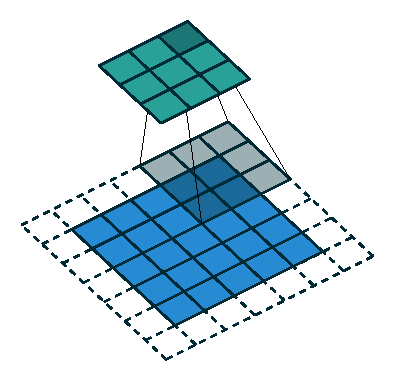
\includegraphics[width=0.24\textwidth]{pdf/padding_strides_02.pdf}
    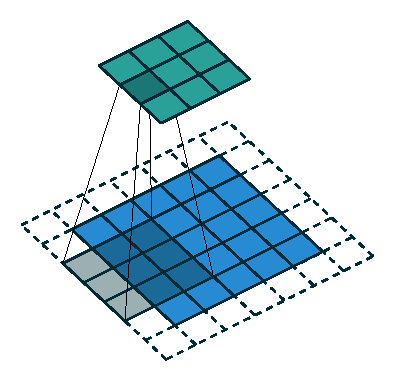
\includegraphics[width=0.24\textwidth]{pdf/padding_strides_03.pdf}
    \caption{\label{fig:padding_strides} 
        Convolving $3 \times 3$ weights over a $5 \times 5$ input with stride=2 and padding=1.}
\end{figure}


\FloatBarrier
\newpage
\section{Pooling}

In addition to discrete convolutions themselves, {\em pooling\/} operations are another important building block in CNNs. 
Pooling operations usually reduce the size of feature maps by using some function to summarize subregions, such as taking the average or the maximum value.

Pooling slides a window across the input, just like a convolution. 
The difference is that instead of multiplying the features in that window by weights, pooling layers feed the features in that layer into a simple \textit{pooling function}. 
The pooling function is usually max or average.
Again, pooling operations have strides and padding that behave in the same way as a standard convolution.
Usually, when pooling we use a stride of at least 2, to ensure that we are actually reducing the size of the feature map (though in the example below we use stride=1).
\begin{figure}[H]
    \centering
    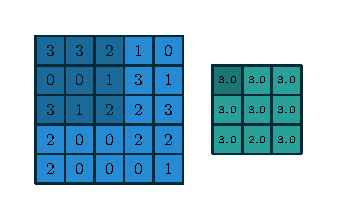
\includegraphics[width=0.32\textwidth]{pdf/numerical_max_pooling_00.pdf}
    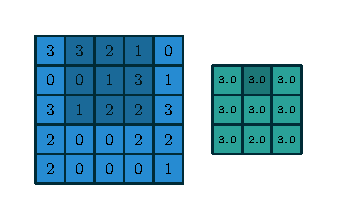
\includegraphics[width=0.32\textwidth]{pdf/numerical_max_pooling_01.pdf}
    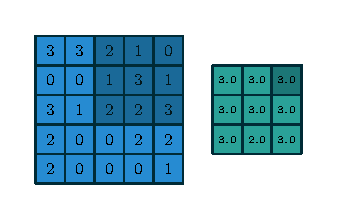
\includegraphics[width=0.32\textwidth]{pdf/numerical_max_pooling_02.pdf}
    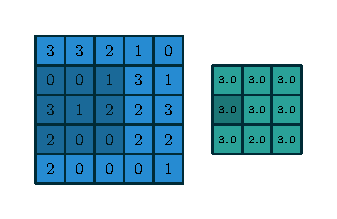
\includegraphics[width=0.32\textwidth]{pdf/numerical_max_pooling_03.pdf}
    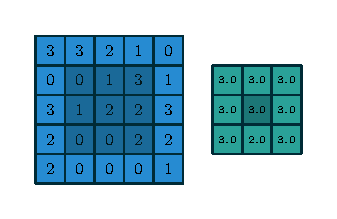
\includegraphics[width=0.32\textwidth]{pdf/numerical_max_pooling_04.pdf}
    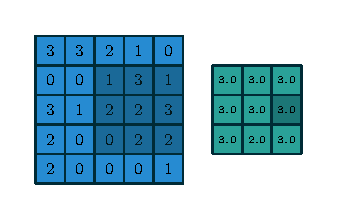
\includegraphics[width=0.32\textwidth]{pdf/numerical_max_pooling_05.pdf}
    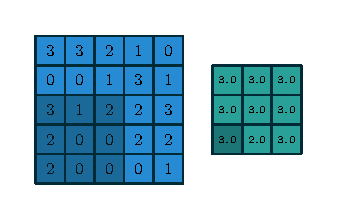
\includegraphics[width=0.32\textwidth]{pdf/numerical_max_pooling_06.pdf}
    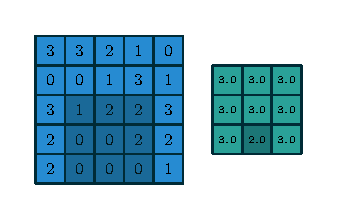
\includegraphics[width=0.32\textwidth]{pdf/numerical_max_pooling_07.pdf}
    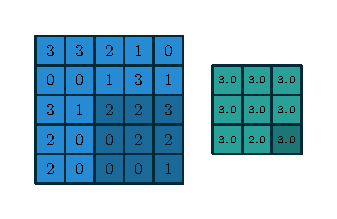
\includegraphics[width=0.32\textwidth]{pdf/numerical_max_pooling_08.pdf}
    \caption{\label{fig:numerical_max_pooling} Max pooling on a $5 \times 5$ input using kernel size=3, stride=1, padding=0}
\end{figure}

\subsection{Global average pooling}

For image classification, we ultimately want just vector of logits as our output (for a single image).
But convolutional layers are going to give us a whole feature map of size $\text{channels} \times \text{height} \times \text{width}$.
So how can we convert a feature map into just a vector?
Perhaps the most common method is ``global average pooling'', which just averages over the spatial dimensions.
\begin{align}
  \text{feature vector}_c &= \tfrac{1}{HW} \sum_{x=1}^W \sum_{y=1}^H \text{feature map}_{c, x, y}
\end{align}
In PyTorch, it is easiest to implement this using \verb|nn.AdaptiveAvgPool2d(1)|, which returns a feature map with height=1 and width=1 (that's what the 1 specifies: if you did \verb|nn.AdaptiveAvgPool2d(3)|, it would return a feature map with height=3 and width=3).

\FloatBarrier
\clearpage
\section{Data Augmentation}
Often I use convolutional neural networks for classification: i.e.\ for classifying what object is present in the image.
Interestingly, it turns out that if I take an image of a kitten, and:
\begin{itemize}
  \item Horizontal flip.
  \item Small rotation.
  \item Small translation/crop.
\end{itemize}
I still end up with an image of a kitten.
\begin{figure}[H]
  \centering
  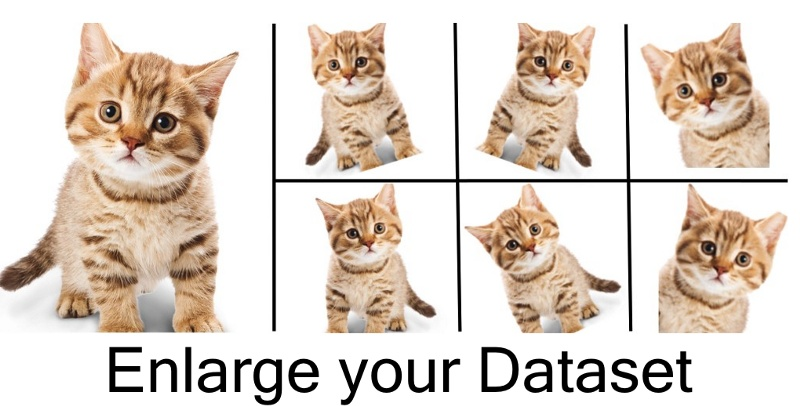
\includegraphics[width=0.8\textwidth]{data_augmentation}
\end{figure}
So I can effectively enlarge my dataset by flipping/rotating/cropping all my images.
And this turns out to be a \textit{huge} factor in the success of modern networks.
Basically all modern networks for images use some form of data augmentation.




\FloatBarrier
\clearpage
\section{Batchnorm}

Batchnorm ensures that each channel has a specified, learned mean and variance.
First, batchnorm computes the mean-and variance across channels, averaging across images in the minibatch, and across spatial locations.
\begin{align}
  \mu_c &= \tfrac{1}{NHW} \sum_{i=1}^N \sum_{x=1}^W \sum_{y=1}^H \text{input}_{i,c,x,y},\\
  \sigma^2_c &= \tfrac{1}{NHW}\sum_{i=1}^N \sum_{x=1}^W \sum_{y=1}^H (\text{input}_{i,c,x,y} - \mu_c)^2.\\
  \intertext{Then, batchnorm ``standardises'' the inputs: subtracting the per-channel mean, and dividing by the per-channel standard deviation,}
  \text{standardised input}_{i,c,x,y} &= \frac{x_{i,c,x,y} - \mu_c}{\sigma_c}.
  \intertext{Importantly ``standardised input'' has mean 0 and standard-deviation 1 for all channels.  This is a bit restrictive: the neural network might perform better if the outputs have a different mean and standard deviation.  Therefore, batchnorm finally multiplies by per-channel scale-factor, $\gamma_c$ and adds a per-channel offset, $\beta_c$,}
  \text{output}_{i,c,x,y} &= \gamma_c \; \text{standardised input}_{i,c,x,y} + \beta_c.
\end{align}
Thus, the outputs of batchnorm have standard deviation $\gamma_c$ and mean $\beta_c$.

There are lots of hypotheses for how batchnorm works, but I haven't really been convinced by any of them.
Suffice it to say that batchnorm seems to stabilise training, and it seems to be \textit{really} important for getting neural networks to work well.
In fact, it gives perhaps the biggest boost to neural network performance of any modification (except perhaps data augmentation, which also makes a huge difference).



\FloatBarrier
\clearpage
\section{Classic convolutional neural networks}

We're now in a position to understand the full architecture of some of the most classic convolutional neural networks (CNNs).
Specifically, we're going to look at arguably the two historically most important two neural networks: LeNet and AlexNet.

LeNet was developed in Yann LeCun et al. in 1998, and was designed to recognise images of handwritten digits (MNIST).
This dataset included 60,000 greyscale, $28\times 28$ images of handwritten digits (we have already seen this dataset).
The resulting system was deployed in the real-world to read millions of checks.
LeNet was the first demonstration that neural networks could do interesting tasks.

AlexNet was developed by Alex Krizhevsky et al. in 2012.
If we have to choose a network that started the ``deep learning revolution'', most people would choose AlexNet.
AlexNet was designed to solve a much, much harder task: recognising one of 1000 objects in large (224 x 224 color images).
Specifically, this dataset is known as ImageNet-1k (as it has 1000 object classes).  
This dataset has about one million training examples.
AlexNet was about 50\% better than the previous best method, based on hand-engineered features.

\begin{figure}[H]
  \centering
  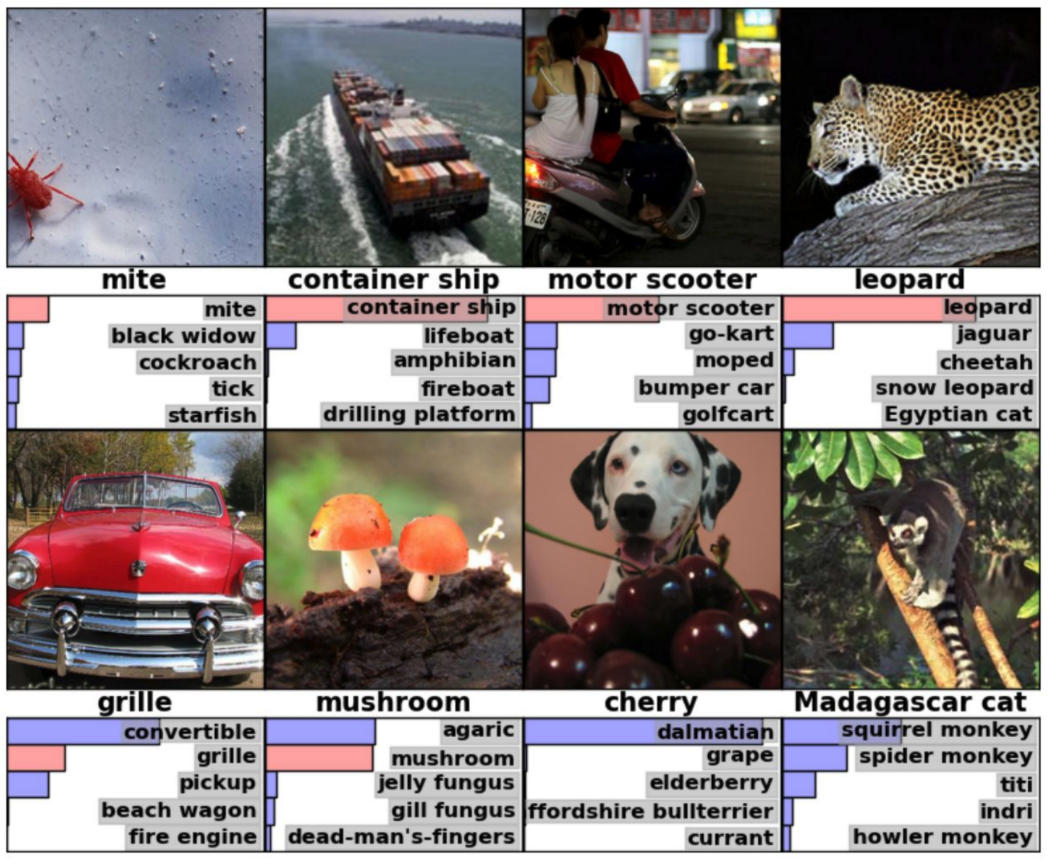
\includegraphics[width=0.8\textwidth]{imagenet}
  \caption{\label{fig:imagenet}
    Examples of images from imagenet, along with their class labels (as given in the dataset), and example classifications from a neural network.
    Note that class-labels are often ambiguous (dalmation vs cherry, convertible vs grille vs pickup, mushroom vs agaric), so 100\% accuracy likely isn't possible.
  }
\end{figure}

Lets zoom in a bit on the architecture (the details of these architectures is non-examinable; I'm not going to ask about the architecture of LeNet / AlexNet; but they are useful for illustrating what these networks typically look like).
\begin{figure}[H]
  \centering
  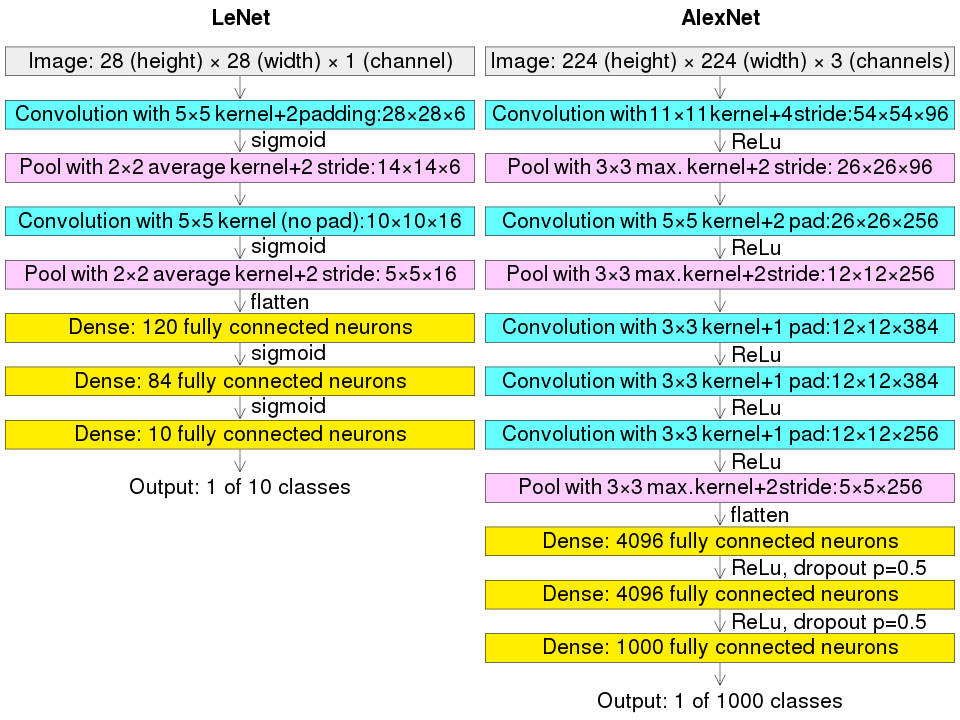
\includegraphics[width=0.8\textwidth]{lenet_vs_alexnet}
  \caption{\label{fig:lenet_vs_alexnet} Each box is a fully-connected (dense), convolutional, or pooling layer.  The size of the output is given in each box after the colon.
  }
\end{figure}
We can see the differences are surprisingly minimal.
AlexNet's success is typically attributed to:
\begin{itemize}
  \item Use of relu rather than sigmoid nonlinearities.  As discussed previously, relu gives better backpropagation of gradients.
  \item AlexNet was one of the first times that GPUs were used to train neural networks, so they were able to use much more compute for training.
  \item Dropout for regularisation.
  \item An early variant of batchnorm after some of the nonlinearities (not shown on the diagram).
  This variant is no longer used, so is not discussed further in this course.
\end{itemize}

\FloatBarrier
\clearpage
\section{Modern convolutional neural networks: ResNets}

Modern convolutional networks have a very similar structure.
The only difference is the addition ``skip connections''.  They're called ``skip'' connections, because skip over a number of layers in the network.
Modern convolutional neural networks with skip connections are typically known as ``ResNets'' or ``Residual Networks''.
A skip connection looks something like:
\begin{figure}[H]
  \centering
  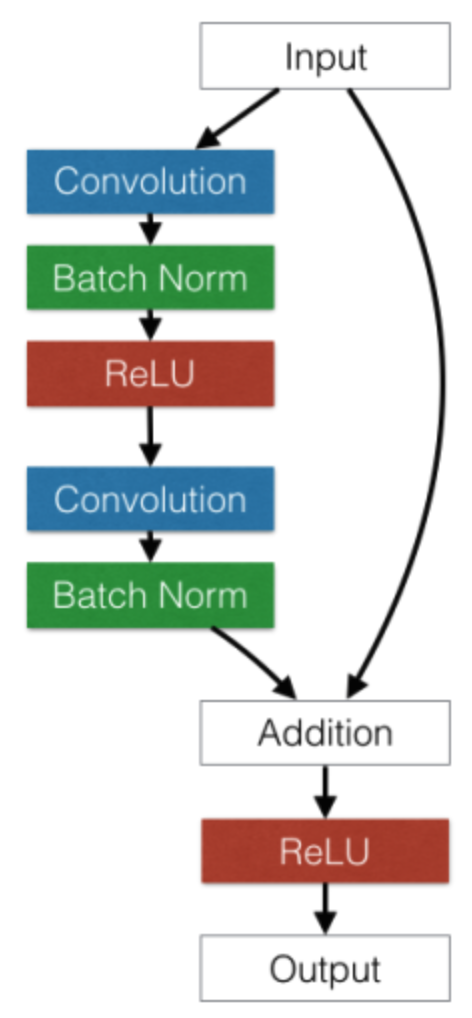
\includegraphics[width=0.3\textwidth]{resnet_block}
\end{figure}
Note the arrow on the right that bypasses the two convolutional layers.
In equations,
\begin{subequations}
\begin{align}
  a_1 &= \text{batchorm}(\text{conv}(\text{input}, ...))\\
  a_2 &= \text{batchorm}(\text{conv}(\text{relu}(a_1), ...))\\
  \label{eq:resnet_output}
  \text{output} &= \text{relu}(\underbrace{\text{input} +}_\text{skip conn.} a_2)
\end{align}
\end{subequations}
Here, the $...$ denotes the parameters of the convolutional layer, i.e.\ the weights and biases.

There is a skip connection in the final expression, Eq.~\eqref{eq:resnet_output}, arising from the use of ``input'' in that expression.
Using ``input'' directly means skipping over all the NN layers used in computing $a_1$ and $a_2$.

Don't worry about the precise details of exactly what order the operations go in: there are \textit{loads} of different variants.
The key idea is just that the skip connections bypass some network layers.

Most of the modern ``backbone'' networks for image tasks use some variant of a ResNet (i.e. a convolutional network with these skip connections.

ResNets seem to work really well, but it isn’t really known why. One idea is that the skip connections help “signal” propagate through the network early on, and thereby help with training.  But again, I'm not hugely convinced by this idea.




\end{document}

